\documentclass[11pt,a4paper]{article}

\usepackage[T1]{fontenc}
\usepackage{amsmath}
\usepackage{amssymb}
\usepackage{graphicx}
\usepackage{booktabs}
\usepackage[margin=25mm]{geometry}
\usepackage[authoryear,round]{natbib}
\usepackage{hyperref}

\hypersetup{
  colorlinks=true,
  linkcolor=black,
  citecolor=black,
  urlcolor=blue
}
\graphicspath{{figures/}}

\title{Validation of a sharp-interface void-bubble solver for long bubbles in
circular tubes}
\author{Vatsal Sanjay}
\date{September 2026}

\begin{document}

\maketitle

\begin{abstract}
A long bubble translating through a wetting liquid in a circular tube deposits
an annular film on the wall. We validate an axisymmetric sharp-interface
finite-element solver for this problem in which only the liquid is meshed, the
bubble interior is a true void of uniform pressure, and the steady state is
obtained in a frame co-moving with the bubble rather than by marching a
laboratory-frame transient. The bubble speed is a global unknown closed by the
void centroid, not a regression against a tip trajectory. Twenty-five
capillary numbers span $1.0\times10^{-4}\le Ca_b\le14.8$, five decades. In the
thin-film limit $H/Ca_b^{2/3}$ extrapolates to $1.3370$, within $0.03$--$0.04\%$
of Bretherton's $0.643\,3^{2/3}=1.3375$, so the asymptotic coefficient is
recovered rather than assumed. The dynamic pressure excess across the front
meniscus independently recovers Bretherton's other coefficient, $3.58$, to
$0.4\%$. At finite capillary number the solver agrees
with the published axisymmetric finite-element results of Giavedoni and Saita
to $+0.12\%$ at $Ca_b=1.0$, $-0.18\%$ at $2.0$ and $+0.05\%$ at $10.0$ (the last
of those is printed text, not a digitised figure). It
departs from the Aussillous--Qu\'er\'e representation of Taylor's measurements
by at most $1.37\%$ anywhere below $Ca_b=2$, with two sign changes, and by
$-4.56\%$ at $Ca_b=14.8$ where that fit is extrapolated far beyond its data.
Fifteen verification stages are reported, including a displacement test showing
the computed state is an attractor rather than merely a fixed point and a
route-independence test showing the curve does not carry its own history.
We also find the rear cap ceasing
to be convex between $Ca_b=1.024$ and $1.048$ in Stokes flow, a bracket
containing the $1.026$ obtained by extrapolating the independent Stokes
correlation of Balestra and co-workers, and we resolve the vortex ring trapped
in the resulting indentation. At the top of the sweep the Stokes film moves by
$0.78\%$ at $Re=1.47$. A companion volume-of-fluid campaign lies above the
present curve by up to $4.6\%$ near $Ca_b=1$; the cause of that difference is
not established, though two candidates are eliminated.
\end{abstract}

\section{Scope}

This report validates one solver. It is a derived workstream of a
volume-of-fluid campaign on the same physical problem, and the two are designed
to be compared point by point; where that comparison appears below, it is
labelled as such and no claim is made about which code is closer to the truth.

Three statements are worth separating at the outset, because they are
established by different evidence and carry different weight. That the discrete
equations are solved accurately is shown by the verification stages of
Section~\ref{sec:verification}, which compare against analytic answers, against
independent solve routes, and against the solver's own refinement. That the
equations being solved are the intended ones is shown by the limiting-case
result of Section~\ref{sec:limit}, which recovers a coefficient the solver was
never given. That the answer is correct at finite capillary number rests on
agreement with an independent published computation, in
Section~\ref{sec:finite}, and is therefore the weakest of the three.

\section{Problem and reference laws}

Let $R_t$ be the tube radius, $R_0$ the volume-equivalent bubble radius, $U_b$
the bubble speed and $\overline U$ the imposed mean liquid speed. With $\mu$
the liquid viscosity and $\sigma$ the surface tension,
\begin{equation}
  H=\frac{h_{\mathrm{flat}}}{R_t},\qquad
  Ca_b=\frac{\mu U_b}{\sigma},\qquad
  Ca_{\mathrm{in}}=\frac{\mu\overline U}{\sigma}.
  \label{eq:definitions}
\end{equation}
The calculation prescribes $Ca_{\mathrm{in}}$; $Ca_b$ is an output. Every
reference law is therefore evaluated at the computed bubble speed, never at the
imposed one.

For a long bubble at vanishing capillary and Reynolds number,
\citet{bretherton1961motion} matched the viscous dynamic meniscus to the static
outer shape and obtained
\begin{equation}
  H_B=0.643\,(3Ca_b)^{2/3}=1.3375\,Ca_b^{2/3}.
  \label{eq:bretherton}
\end{equation}
The rounded coefficient $1.34$ is conventional and is used in the companion
campaign's tables. The unrounded value is used throughout this report and in
every figure, because the deviations discussed here are as small as $0.2\%$ and
the two conventions differ by about that much in the thin-film limit. Where the
companion data are plotted, their deviations are recomputed from the raw $H$
and $Ca_b$ against Eq.~\eqref{eq:bretherton}, so that no part of any difference
between the two codes is an artefact of the prefactor.

At finite capillary number \citet{aussillous2000quick} represented the
circular-tube measurements of \citet{taylor1961deposition} by the Pad\'e form
\begin{equation}
  H_T=\frac{H_B}{1+R\,H_B},\qquad R=2.5.
  \label{eq:aq}
\end{equation}
This is an empirical fit, not a solution of the governing equations, and its
range of support is set by Taylor's data. \citet{klaseboer2014extended}
re-derived the same functional form from a matched spherical-cap construction
and prefer $R=2.79$. Equation~\eqref{eq:aq} is used below as a reference curve
that makes small differences visible, and not as a standard of correctness;
Section~\ref{sec:finite} reports where it ceases to represent the computed film.

Bretherton's second observable follows from mass conservation. If the deposited
film is at rest in the laboratory frame, then
\begin{equation}
  \frac{Ca_b}{Ca_{\mathrm{in}}}=\frac{1}{(1-H)^2},
  \qquad m=1-(1-H)^2,
  \label{eq:stagnant}
\end{equation}
with $m$ the fraction of liquid left behind. Equation~\eqref{eq:stagnant} is
used here as a diagnostic, not as an input: the solver computes $Ca_b$, $H$ and
the fluxes independently, and the residual in Eq.~\eqref{eq:stagnant} is
reported rather than enforced. A film that is genuinely not stagnant is
physics, not error.

\section{Formulation}

The solver computes axisymmetric Stokes or Navier--Stokes flow in the liquid
alone, with a sharp free surface carrying surface tension. Three choices
distinguish it from a laboratory-frame two-phase calculation of the same
problem, and each is load-bearing.

\paragraph{The bubble interior is a void.} No gas domain is meshed and no
volume-of-fluid field exists. Surface tension acts on the liquid--void
interface, whose nodes are mesh nodes, so the interface is not reconstructed
from a colour function and the film thickness is read directly off the
discretisation rather than inferred from it. The interior pressure is uniform.

\paragraph{The bubble volume is fixed and the void pressure is its Lagrange
multiplier.} The void pressure is not zero. The cap curvature of a confined
bubble is set geometrically at roughly $2/(R_t-h)$, so the normal-stress
balance determines the interior pressure from the local liquid pressure;
changing the volume changes the bubble's length, not its cap curvature. With
the interior pressure pinned instead and the volume left free, the computed
volume would track the axial pressure drop and hence the window length, which
is the very dependence the co-moving formulation exists to remove. Fixed volume
is also the faithful analogue of an incompressible gas phase.

\paragraph{The frame co-moves with the bubble and its speed is an unknown.} In
a laboratory frame the domain must be long enough to contain the trajectory,
and the steady state is a transient sampled when a stopping criterion fires. In
the co-moving frame the bubble does not translate through the mesh; the window
need only be long enough for the cap disturbance to decay to the fully
developed profile, and the steady equations are solved directly. The frame
speed $U_b$ enters as a global degree of freedom closed by requiring the void's
axial first moment to be stationary. Because the fully developed solution in a
circular tube \emph{is} Poiseuille flow, imposing it at both ends is the
infinite-tube condition rather than an approximation to it.

The working nondimensionalisation is $\sigma=\mu=R_0=1$, so $Ca_{\mathrm{in}}$
is the imposed mean inlet speed and the Laplace number $La=\rho$. All results
below are at $La=0$, that is, Stokes flow, with $R_t/R_0=0.7$ and bubble volume
$\tfrac43\pi R_0^3$. Section~\ref{sec:verification} reports the measured size
of the inertial correction at $La=1$ on the thin-film state, and
Section~\ref{sec:open} quotes the Reynolds bound measured at the top of the
sweep.

The implementation uses pyoomph \citep{diddens2024bifurcation}, which is built
on \texttt{oomph-lib} \citep{heil2006oomph} and GiNaC \citep{bauer2002ginac},
with Taylor--Hood elements for the flow and a hyperelastically smoothed moving
mesh. Problem sizes range from $1.1\times10^4$ to $3.7\times10^5$ degrees of
freedom.

\section{Verification}
\label{sec:verification}

Table~\ref{tab:stages} lists the staged checks. A stage earns its place by
being able to fail: restating how well Newton converged is not a check, so
every stage below compares against something the solver did not choose---an
analytic answer, an independent route to the same state, a different
discretisation, or a limit in which the answer is known.

\begin{table}[t]
  \centering
  \caption{Verification stages. Each is a script that exits non-zero on failure
  and writes a machine-readable receipt. Numbering has gaps because three
  intermediate stages were folded into the production path during development.}
  \label{tab:stages}
  \small
  \begin{tabular}{@{}lp{50mm}p{72mm}@{}}
    \toprule
    Stage & Question & Result \\
    \midrule
    S0 & Does the bare window reproduce Poiseuille flow? & Flux to $4.4\times10^{-16}$, pressure drop to $5.0\times10^{-14}$, worst of four configurations \\
    S1 & Does an unconfined void relax to a sphere at the Laplace pressure? & Radius to $1.1\times10^{-5}$, interior pressure to $2.2\times10^{-6}$ \\
    S5 & Is the answer independent of the window length? & See below \\
    S6 & Is it independent of the mesh? & $H$ moves by at most $7.9\times10^{-5}$ relative \\
    S7 & Does the pressure datum affect any observable? & Two mechanisms agree to $2.6\times10^{-14}$ \\
    S8 & How large is the inertial correction? & $-0.0255\%$ in $H$ between $La=0$ and $La=1$ at one $Ca$ \\
    S9 & Is the computed state an attractor? & Displacements decay to $0.03$--$0.57\%$ in $1.5$ film renewals \\
    S10 & Does the answer depend on the solve route? & Routes agree to $9.1\times10^{-5}$; retrace to $8\times10^{-13}$ \\
    S11 & Where does the rear cap stop being convex? & Onset in $1.024<Ca_b<1.048$; resolutions agree above $4\times10^{-4}R_t$ \\
    S12 & Does azimuthal eigensolving work on this problem? & Runs for every mode tested; rightmost eigenvalue converged in the number requested; reference state stable \\
    S13 & Does the rightmost eigenvalue match a time march? & Period to $2\times10^{-16}$; decay rate to $5\%$ (film envelope) and $14\%$ (velocity) \\
    S15 & To what $Re$ may the Stokes baseline be quoted? & Holds to $0.78\%$ for $Re<1.47$ \\
    S16 & Does the pressure datum move the axisymmetric spectrum? & Rightmost $\lambda$ agrees; $Ca_b$ spread $5.0\times10^{-14}$ \\
    S17 & Does $La=1$ continuation past $Ca_{\mathrm{in}}=2.91$ survive with remesh off? & No; it dies at $2.90851$ with the mesh unchanged. Continuation limit \\
    S19 & What is $H$ on the named $(Ca_{\mathrm{in}},La)$ grid? & Stokes quote unchanged for $Re<1.47$; $La=10$ at $Ca_{\mathrm{in}}=0.5$ thins $H$ by $5.8\%$ \\
    \bottomrule
  \end{tabular}
\end{table}

Three of these deserve comment, because they test things a residual norm cannot.

\paragraph{Window independence is tested by the quantity that would expose it.}
Rather than refining the pad and observing that the answer stops moving, S5
compares the exact Poiseuille outlet with a traction-free one at the same pad.
If the window is effectively infinite the outlet condition cannot matter, so
this gap must collapse faster than either condition converges alone. At
$Ca_{\mathrm{in}}=0.05$ the relative gap in $H$ is $1.29\times10^{-3}$,
$5.1\times10^{-6}$ and $3.0\times10^{-11}$ at pads of one, two and five tube
radii: eight orders against four for the individual convergence. Varying the
pads separately shows that the \emph{front} pad controls and the rear does not,
by a factor of about $600$ at pad one. This is the Landau--Levich geometry: in
the bubble frame the wall moves rearward, so the advancing front meniscus is
the coating meniscus that sets the film and the rear meniscus only receives it.
A symmetric-only study would have concealed this.

\paragraph{Steadiness is tested by displacement, not by persistence.} The
reported states come from a stationary solve, which is an exact fixed point of
the implicit time discretisation as well as of the steady equations. Marching
from such a state therefore leaves it in place to round-off whether it is an
attractor or a saddle, and persistence alone shows almost nothing. S9 instead
displaces the state---to the converged solution at a capillary number $5\%$
away, then restores the parameter---and marches in time alone with no
stationary polish. The imposed interface displacement of $4.6\times10^{-4}$ to
$3.6\times10^{-3}$ in $r/R_t$ decays to between $0.03\%$ and $0.57\%$ of itself
within $1.5$ film renewals, and $H$ returns to within $1.4\times10^{-5}$.

The horizon of that test is quoted in film renewals $L_b/U_b$ rather than in
capillary times, and deliberately. That renewal time is $3172$ time units at
$Ca_b=1.0\times10^{-3}$ and $0.51$ at $Ca_b=14.8$, a factor of six thousand
across the sweep, so a single nondimensional horizon quoted uniformly would
claim four orders of magnitude more evidence at one end than at the other.

\paragraph{The curve is not allowed to carry its own history.} Points up to
$Ca_{\mathrm{in}}=0.7$ are each solved from their own seeded shape,
independently of their neighbours; above that they come from an ascending
continuation ladder, because a fresh transient costs a full relaxation per
point where a continued step costs under a second. That switch is a matter of
cost and not of capability: S10 measures a fresh solve succeeding as high as
$Ca_{\mathrm{in}}=2$, that is $Ca_b=4.79$. Where both routes work they agree to
$9.1\times10^{-5}$ in $Ca_b$ and $8.2\times10^{-5}$ in $H$, and walking the
ladder up to $Ca_{\mathrm{in}}=6$ and back down returns the same states to
$8\times10^{-13}$.

S10 also varies the bubble's length at fixed volume, by changing $R_t/R_0$ from
$0.7$ to $0.5$. This lengthens the bubble by a factor of $1.8$ and moves $H$ by
$1.3\times10^{-3}$ at $Ca_b=0.011$, falling to $1.9\times10^{-4}$ at
$Ca_b=0.585$. The effect survives doubling the film resolution, which changes
each confinement by about $10^{-5}$ and leaves the difference at
$1.33\times10^{-3}$, so it is a resolved finite-bubble effect and not a
discretisation error. It also bounds how much of any cross-code difference
could be attributed to a mismatch in $R_0/R_t$.

Across the production sweep the void volume is conserved to at most
$2.1\times10^{-8}$ and the residual in the stagnant-film identity,
Eq.~\eqref{eq:stagnant}, reaches at most $6.0\times10^{-4}$. The latter couples
the frame speed, the film thickness and the flux in one relation and would fail
if any of them were wrong; it is a consistency check on mass conservation and
film flatness, and it is not by itself evidence that $H$ is correct.

S16 checks that the two pressure datums agree on the rightmost axisymmetric
eigenvalue at $Ca_{\mathrm{in}}=0.05$. The pair is
$-0.123205\pm0.157796\,\mathrm{i}$ under nodal fixation and under the
integral datum; the base states agree in $Ca_b$ to $5.0\times10^{-14}$.

\section{The Bretherton limit}
\label{sec:limit}

A line of slope $2/3$ over a moderate range does not establish the asymptotic
coefficient. The test is whether $H/Ca_b^{2/3}$ tends to $1.3375$ as
$Ca_b\to0$, and at the smallest capillary number computed here the ratio is
$1.3252$, still $0.92\%$ short. That shortfall is not a discrepancy: the
leading confinement correction is itself of order $Ca_b^{2/3}$, so
\begin{equation}
  \frac{H}{Ca_b^{2/3}}\simeq H_B'-R\,H_B'^2\,Ca_b^{2/3}+\cdots,
  \qquad H_B'=1.3375,
  \label{eq:expansion}
\end{equation}
and the ratio must be extrapolated rather than read off. Fitting
Eq.~\eqref{eq:expansion} linearly to the two smallest points gives an intercept
of $1.33697$, which is $0.039\%$ below Bretherton's coefficient; a quadratic fit
to the five smallest gives $1.33707$, or $0.032\%$ below. The solver therefore
recovers a number it was never given, to better than one part in two thousand.

\paragraph{A second coefficient, from a different observable.} The film is not
the only quantity Bretherton predicts, and agreement on one observable does not
imply agreement on another. The pressure excess of the bubble over the liquid
ahead of it is
\begin{equation}
  \Delta p_{\mathrm{front}}
  =\frac{2\sigma}{R_t}\left[1+1.79\,(3Ca_b)^{2/3}\right]
  =\frac{2\sigma}{R_t}+\frac{3.58\,\sigma}{R_t}(3Ca_b)^{2/3}.
  \label{eq:pressure}
\end{equation}
The coefficient $3.58$ is the \emph{leading-meniscus} correction quoted in
Bretherton's abstract; it is not the $4.52$ that applies across a complete long
bubble, front and rear together, and the two must not be interchanged. The
quantity computed here is the front-meniscus excess: the void pressure less the
liquid pressure at the front tip station, obtained by removing the Poiseuille
drop between that station and the outlet, which is window-dependent by
construction and has nothing to do with the bubble. Forming
$(\Delta p_{\mathrm{front}}-2\sigma/R_t)\,R_t/(3Ca_b)^{2/3}$ and extrapolating
as before gives $3.594$ from the two smallest points and $3.569$ from the three
smallest, bracketing $3.58$ within $0.4\%$. This is an independent limiting-case
check: it constrains the normal-stress balance and the void pressure, neither of
which the film thickness alone tests.

The same fit returns the coefficient of the first finite-capillary-number
correction. The initial slope corresponds to $R=2.94$ from the three smallest
points, drifting to $R=2.72$ when five are used. This is to be compared with
$R=2.5$ in the Aussillous--Qu\'er\'e fit and $R=2.79$ preferred by
\citet{klaseboer2014extended}. The measured thin-film value sits above both.
Fitting Eq.~\eqref{eq:aq} with $R$ free over the whole sweep gives $R=2.67$
with a root-mean-square residual of $3.6\%$, so no single value of $R$
represents five decades; this is the quantitative form of the statement that
Eq.~\eqref{eq:aq} is an interpolation over a finite range.

\section{The deposited film at finite capillary number}
\label{sec:finite}

Figure~\ref{fig:film} shows the computed film over five decades against the
reference laws, the digitised axisymmetric finite-element results of
\citet{giavedoni1997axisymmetric}, and the companion volume-of-fluid campaign.
The tabulated data are supplied in \nolinkurl{data/film-sweep.csv}.

\begin{figure}[t]
  \centering
  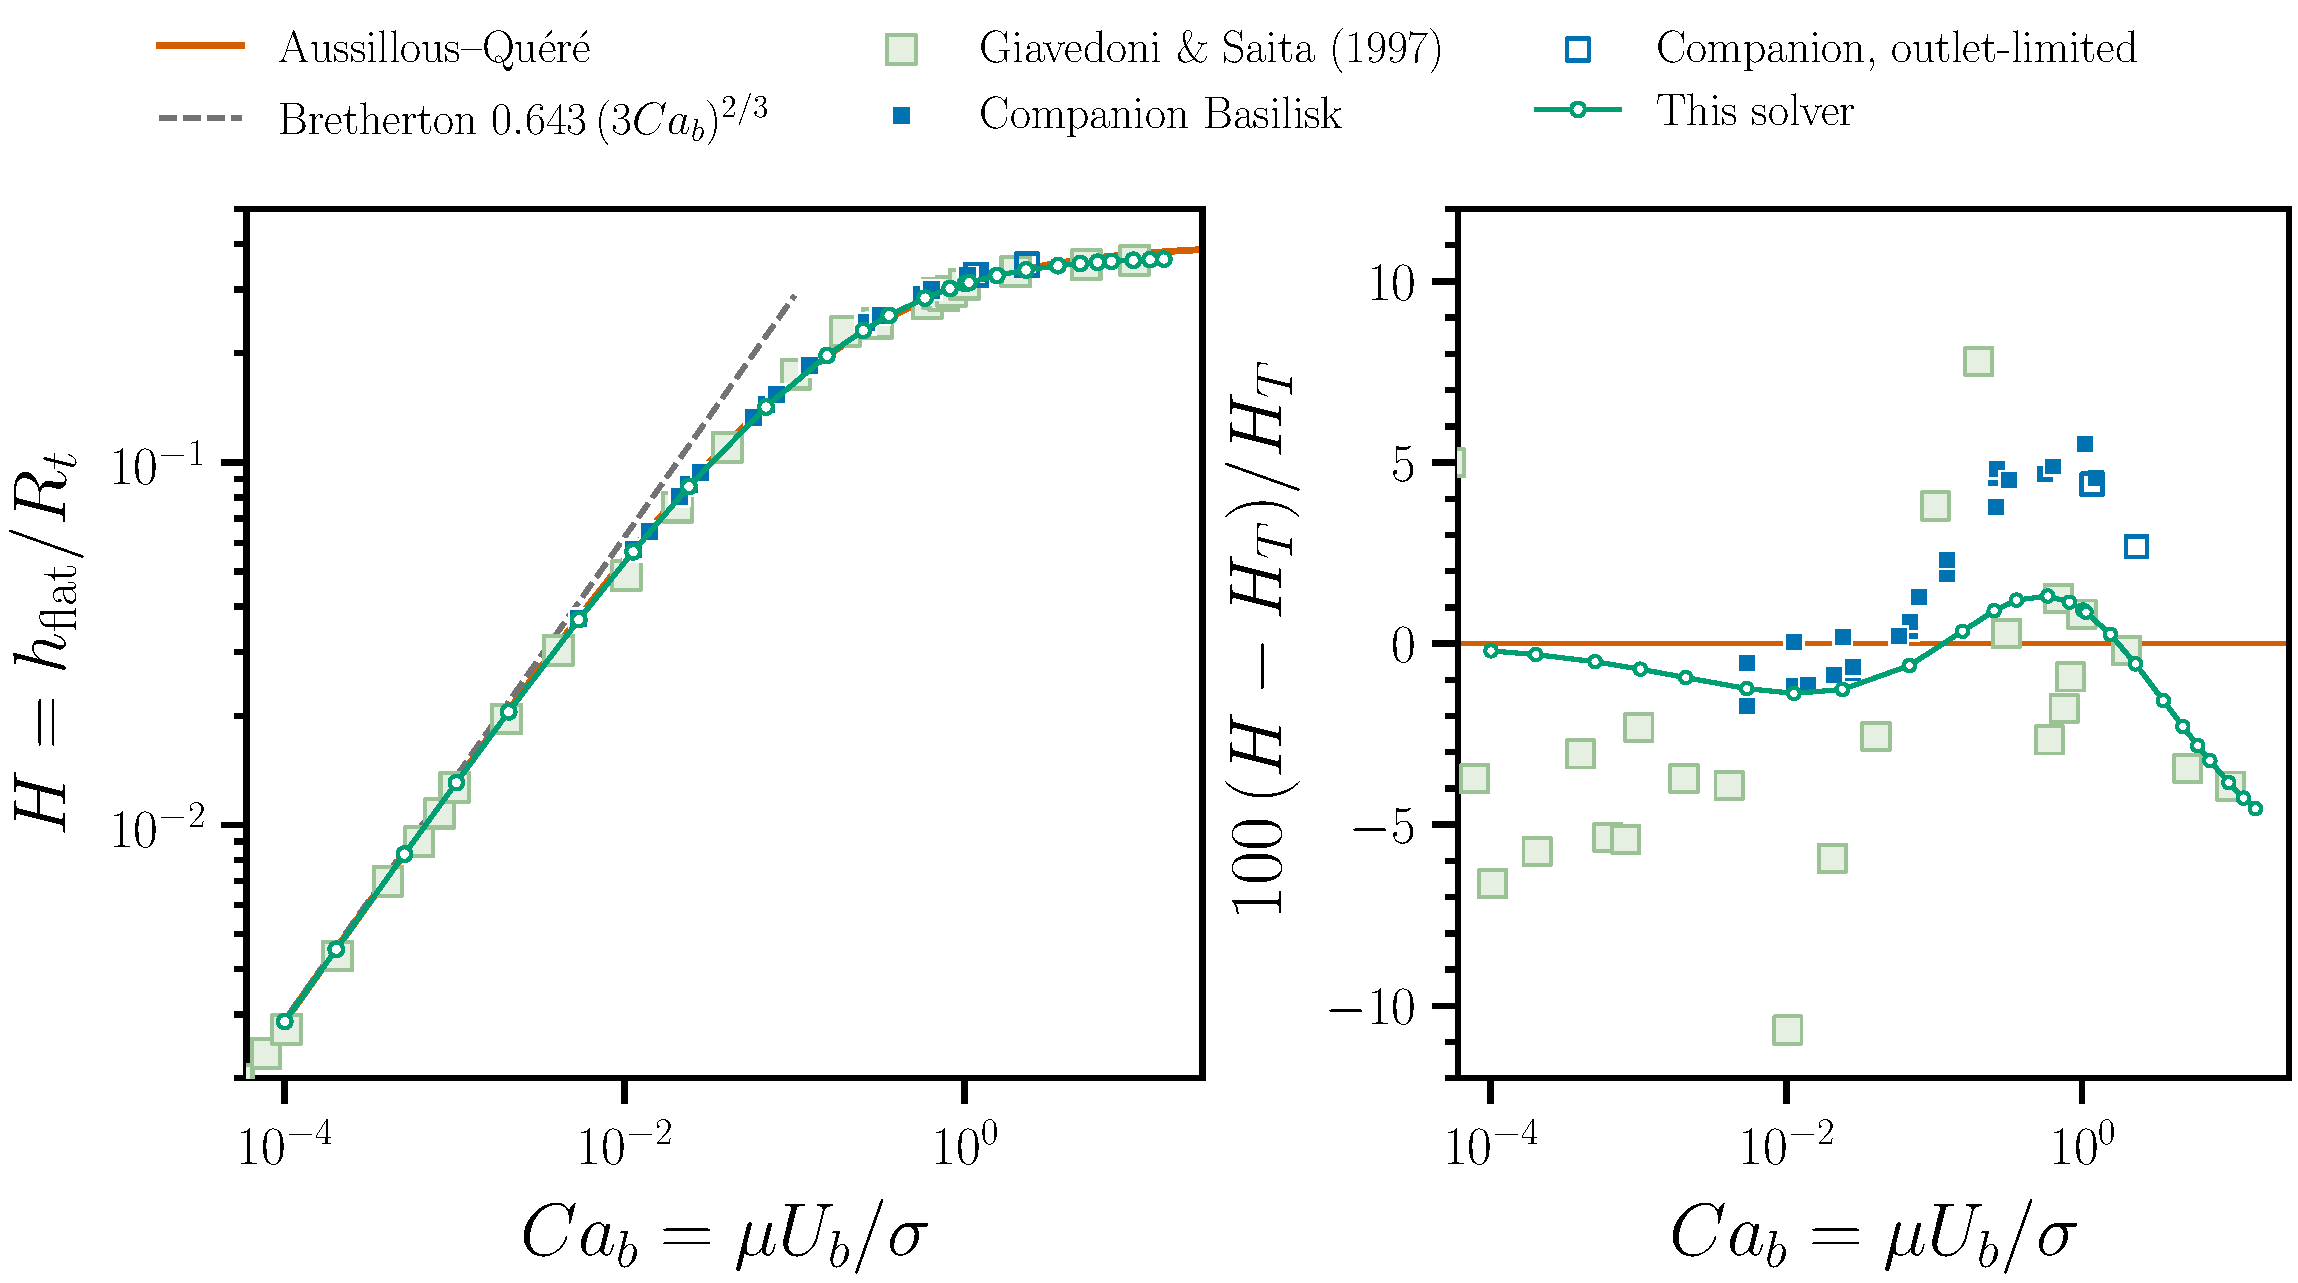
\includegraphics[width=\textwidth]{film-thickness-vs-ca.pdf}
  \caption{Deposited central film against the computed bubble capillary number.
  Left: $H$ with the Bretherton asymptote and the Aussillous--Qu\'er\'e fit.
  Right: the deviation of every series from that fit, all recomputed from raw
  $H$ and $Ca_b$ against the unrounded coefficient of
  Eq.~\eqref{eq:bretherton}. Most literature points are digitised from figures
  and are drawn as large soft symbols for that reason; their scatter at small
  $Ca$ is reading error, not disagreement. The points at $Ca=2$ and $Ca=10$
  are printed values from the same paper. Two companion cases reached the end
  of their laboratory-frame domain and are drawn open.}
  \label{fig:film}
\end{figure}

\paragraph{Departure from the empirical fit.} The deviation from
Eq.~\eqref{eq:aq} is $-0.20\%$ at $Ca_b=1.0\times10^{-4}$ and shrinks
monotonically towards zero as $Ca_b$ falls, as it must if
Section~\ref{sec:limit} is right. Going up in capillary number it reaches a
minimum of $-1.37\%$ at $Ca_b=0.011$, changes sign near $Ca_b=0.115$, reaches a
maximum of $+1.31\%$ at $Ca_b=0.585$, changes sign again near $Ca_b=1.75$, and
then falls monotonically to $-4.56\%$ at $Ca_b=14.8$. Nowhere below $Ca_b=2$
does it exceed $1.37\%$. Mesh convergence is $7.9\times10^{-5}$, two orders below
this structure, so the two sign changes are resolved features of the solution
and not numerical noise. Their interpretation is that a one-parameter Pad\'e
fit cannot follow the true curve over five decades, which is the same
conclusion the free-$R$ fit of Section~\ref{sec:limit} reaches by another
route. We do not interpret the $-4.56\%$ at $Ca_b=14.8$ as an error in either
the solver or the fit: it is the fit being extrapolated an order of magnitude
beyond the data it represents.

\paragraph{Agreement with an independent computation.} The closest available
independent check is \citet{giavedoni1997axisymmetric}: the same geometry, the
same formulation class, a different implementation, and published. Twenty-two
of their twenty-four points fall inside the present range; $Ca=2$ and $Ca=10$
are printed ($m=0.559$ and $m=0.592$, $h_\infty=0.361$ on p.~2424), the rest
digitised from figures.
Interpolating the present sweep onto them, the difference is $+0.12\%$ at
$Ca=1.0$, $-0.18\%$ at $2.0$, $+1.00\%$ at $5.18$ and $+0.05\%$ at $10.0$;
over the nine points with $Ca\ge0.3$ the mean difference is $+1.16\%$ with a
root-mean-square of $1.84\%$. Below $Ca\approx0.05$ the differences widen to
several per cent, which is the expected consequence of reading a thin film off
a logarithmic figure: a fixed pixel error becomes a large relative error as the
film thins. This agreement is the single strongest piece of evidence in this
report that the finite-capillary-number film is right, and it should be read as
consistency across several independent points rather than as a calibration.

\paragraph{Comparison with the companion campaign.} The companion
volume-of-fluid calculations lie above the present curve, by a mean of
$+0.71\%$ below $Ca_b=0.05$, $+2.47\%$ between $0.05$ and $0.3$, and $+3.85\%$
above $0.3$, reaching $+4.6\%$ near $Ca_b=1$. The two curves therefore agree in
the thin-film limit and separate as the film thickens, and over the range where
the literature points are reliable the present curve sits with them. The cause
of the difference is \emph{not established}. Two candidates have been
eliminated. Inertia is not responsible: S8 measures the film moving by
$-0.0255\%$ between $La=0$ and the companion's $La=1$ at $Ca_b=0.068$, and S15
finds at most $0.78\%$ anywhere with $Re<1.47$, both far below the gap. A
mismatch in bubble length is not responsible: S10 bounds its effect at
$1.3\times10^{-3}$. Two candidates remain, and they are distinguishable by
calculations that do not exist yet. The companion's bubble is a viscous gas
with $\mu_g/\mu_c=10^{-2}$ where the present interior is a true void, which is
a genuine physical difference whose size is unknown. The companion also has no
completed spatial refinement sequence, and its stopping rule accepts a film
after an advance of order one bubble radius, which is a fraction of one film
renewal at these capillary numbers. Settling this requires a refinement
sequence and a longer-running case on the volume-of-fluid side; nothing on the
present side can substitute for either.

\section{The rear cap}
\label{sec:rear}

Figure~\ref{fig:rear} shows converged bubble profiles at one capillary number
per decade, and the indentation of the rear cap against $Ca_b$. At low
capillary number the rear cap is convex and carries the familiar capillary
ripple where it joins the film. Above $Ca_b\approx1$ the cap ceases to be
convex: the on-axis rear tip moves \emph{ahead} of the rearmost point of the
interface, so that the bubble's trailing surface folds back around an
axisymmetric indentation. We measure that indentation as
$\delta_{\mathrm{tail}}=z_{\mathrm{tip}}-\min z$ over the rear cap.

\begin{figure}[t]
  \centering
  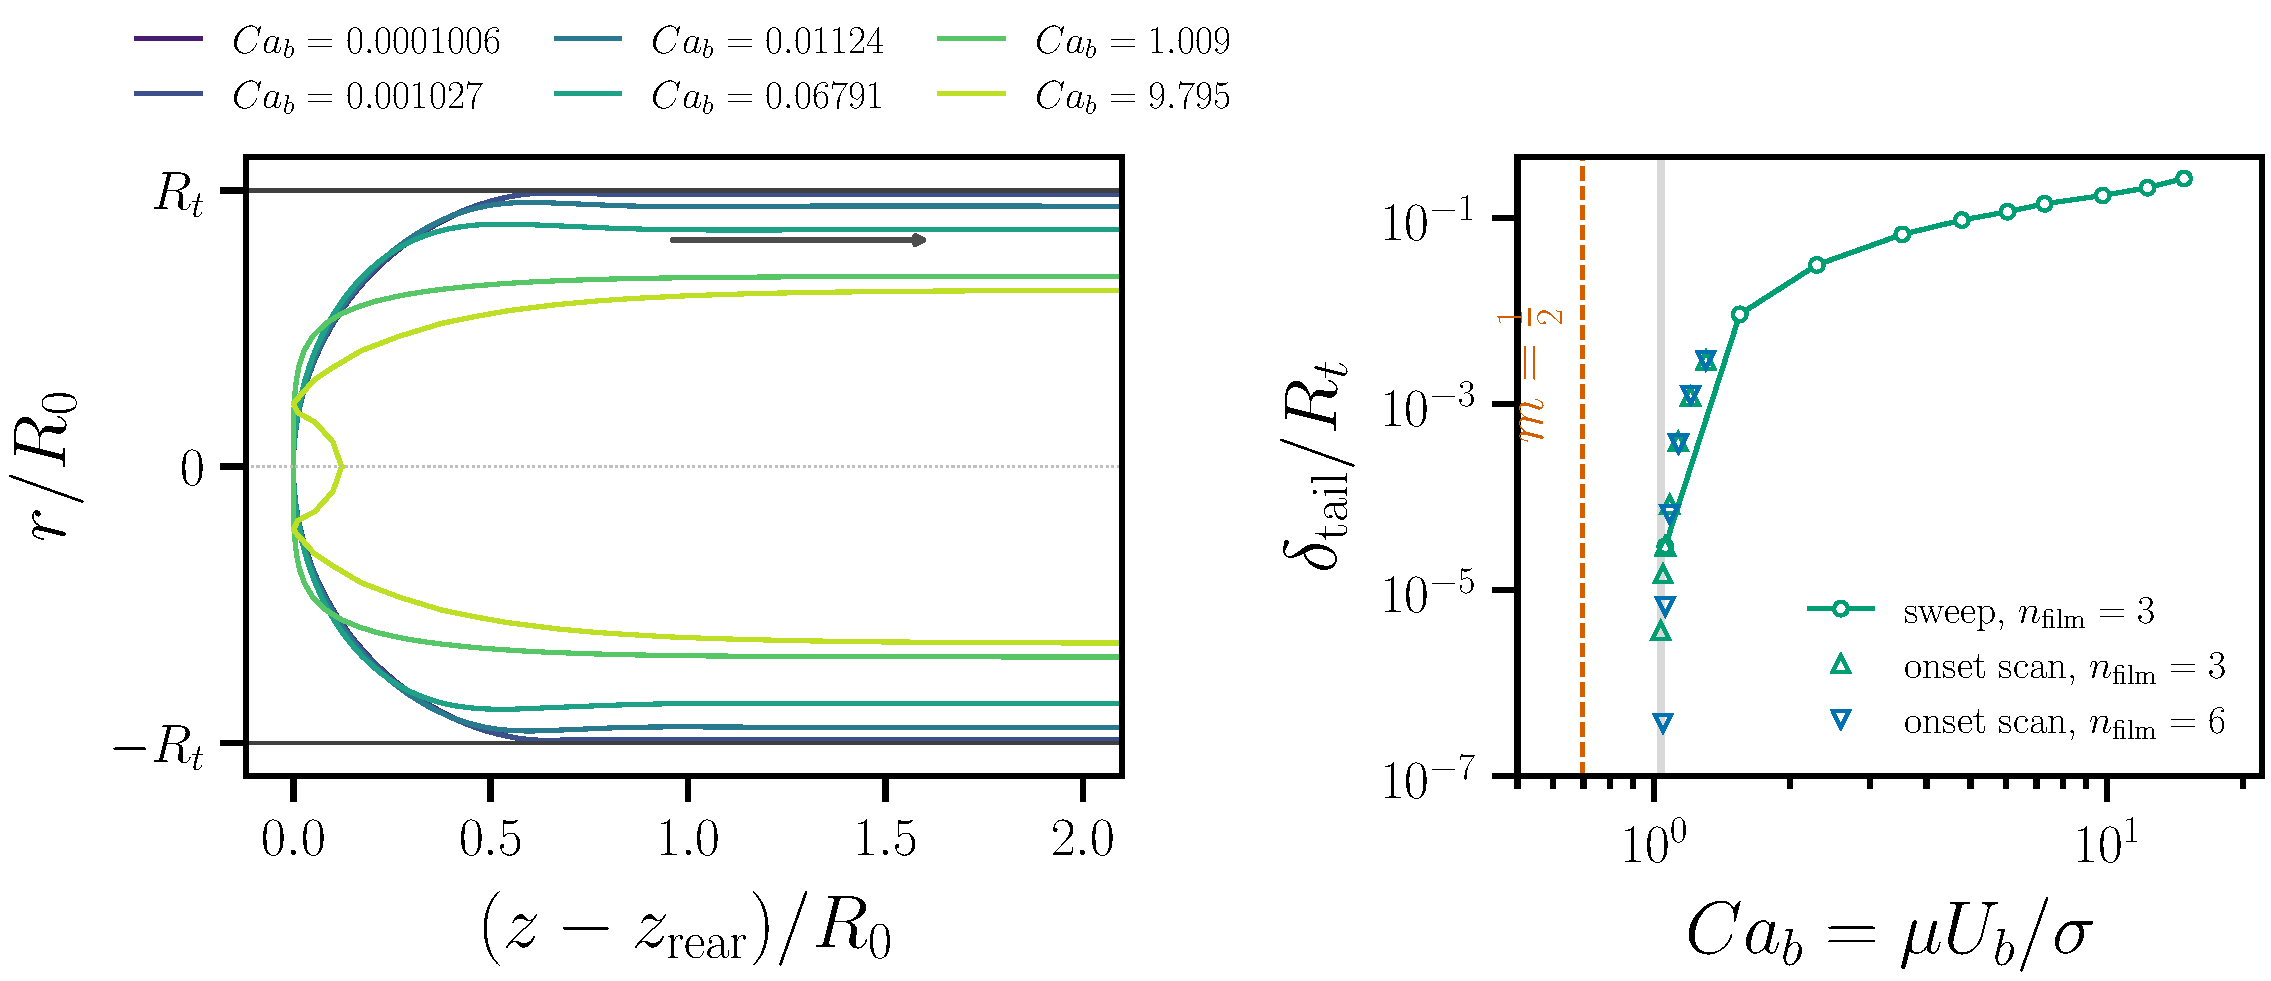
\includegraphics[width=\textwidth]{rear-cap.pdf}
  \caption{Left: converged interfaces, one per decade, each shifted to place its
  rearmost point at the origin and mirrored about the axis; the arrow gives the
  direction of bubble motion. Right: the rear-cap indentation, at two film
  resolutions. Below the shaded band the cap is strictly convex at both
  resolutions and the indentation is identically zero; within the band the two
  resolutions disagree by factors of four to forty, so the band is where the
  cap changes character and not a resolved onset. The dashed line marks
  Taylor's $m=\tfrac12$ condition, which this solver places at $Ca_b=0.695$ and
  which is a distinct and earlier transition.}
  \label{fig:rear}
\end{figure}

\paragraph{The onset is bracketed, not resolved.} At both film resolutions the
cap is strictly convex up to $Ca_b=1.024$, and both give a non-zero
indentation from $Ca_b=1.048$ onwards, so the onset lies in
$1.024<Ca_b<1.048$. It cannot be located more sharply than that: through
$Ca_b\approx1.1$ the two resolutions disagree by factors of four to forty,
which is the signature of an indentation at the level of the discretisation
rather than of the solution. Once
$\delta_{\mathrm{tail}}$ exceeds about $4\times10^{-4}R_t$, at $Ca_b\gtrsim1.1$,
the two resolutions agree to $5\%$ and to $3\%$ beyond that. The indentation
then grows monotonically to $0.27R_t$ at $Ca_b=14.8$. All of this is at
$La=0$, so inertia plays no part in it.

\paragraph{It is a separate transition from Taylor's.} Far from the bubble the
axial velocity on the axis in the bubble frame is
$2\overline U-U_b$, which changes sign when $Ca_b/Ca_{\mathrm{in}}=2$, that is
when $m=\tfrac12$: below it the liquid on the axis outruns the bubble and
recirculates ahead of the nose, above it every streamline moves rearward in the
bubble frame and the flow is complete bypass. Using Eq.~\eqref{eq:stagnant},
that condition is $H=1-1/\sqrt2=0.2929$, and the present sweep crosses it at
$Ca_b=0.695$. The rear cap is still convex there and remains so for a further
$50\%$ in capillary number. The two transitions are therefore ordered and
distinct, and the bypass condition is not sufficient for the indentation. The
computed $m$ rises to $0.595$ at $Ca_b=14.8$.

\paragraph{This reproduces a published Stokes-flow prediction.} A re-entrant
rear cap in a tube at vanishing Reynolds number is not new, and the critical
capillary number is not new either. \citet{martinez1990axisymmetric} predicted
the onset of a re-entrant cavity at the trailing end of a drop at $Ca\approx
0.75$ by boundary integrals; \citet{olbricht1992deformation} observed an
indentation that entrains outer liquid for low viscosity ratio;
\citet{lac2009motion} and \citet{nath2017migration} find the same feature, the
former reporting eventual breakup through a rear re-entrant jet.

The sharpest comparison is \citet{balestra2018viscous}, who solve the
axisymmetric Stokes equations for a confined droplet and fit the plane
curvature of the rear cap as
\begin{equation}
  \kappa_r R=\frac{1+T_r(3Ca_b)^{2/3}}{1+Z_r(3Ca_b)^{2/3}},
  \label{eq:rearcurv}
\end{equation}
with the capillary number built on the \emph{droplet} velocity, as ours is. At viscosity ratio
zero their tabulated coefficients give $T_r=-0.4725$, so the rear curvature
changes sign where $(3Ca_b)^{2/3}=1/0.4725$, that is at $Ca_b=1.026$. Our
bracket, $1.024<Ca_b<1.048$, contains that value.

Three things limit how much weight that agreement carries, and they should be
read before it is quoted. The root is obtained by extrapolating their
correlation to the edge of, and arguably just beyond, the capillary-number
range over which it was fitted, so it is not a value they compute and report.
It is derived from their tabulated coefficients rather than printed by them,
and therefore inherits whatever error the fit carries. And their droplet
volume, $12.9R^3$ against our $12.2R_t^3$, is close but not identical. What can
fairly be said is this: two independent Stokes solvers, neither tuned to this
transition, place it within about one per cent of each other. That is
consistency, and it is the right weight to give it.

The same source predicts the other transition. Their $\lambda=0$ film law with
$Q=2.483$ reaches $H=1-1/\sqrt2$ at $Ca_b=0.720$, against the $0.695$ measured
here, a difference of $3.4\%$. The ordering of the two transitions is worth
recording, because \citet{balestra2018viscous} state in prose that the rear
recirculation detaches at a film thickness \emph{smaller} than the
complete-bypass value, while their own $\lambda=0$ fit puts curvature reversal
at $H=0.311$ and bypass at $H=0.293$, the other way round. Our two independent
measurements, $0.695$ then $1.024$--$1.048$, agree with their model and not
with their prose.

\paragraph{What Giavedoni and Saita do and do not contain.} We cite
\citet{giavedoni1997axisymmetric} for the film data of
Section~\ref{sec:finite}, and it is worth being precise about what else that
pair of papers supports. The 1997 calculation is of a semi-infinite gas finger
with a single advancing meniscus, so it has no rear cap to invert; the
recirculating pattern its abstract reports as overlooked is therefore not a
rear-cap phenomenon. \citet{giavedoni1999rear} adds the trailing meniscus, and
does report a rear-meniscus curvature change --- but at finite Reynolds
number, with the critical capillary number falling as inertia grows. We
therefore exclude that pair as precedent for the \emph{inertialess} inversion
reported here, and not as precedent for the phenomenon at large.

\paragraph{What is not already published.} Two things, both modest. We have
found no published measurement of the indentation \emph{depth} against
capillary number, in any geometry; the monotone growth to $0.27R_t$ at
$Ca_b=14.8$ in Figure~\ref{fig:rear} appears to be new. And the steady branch
is continued an order of magnitude beyond where the prior studies stop: they
terminate near onset because their bubbles break up, whereas a fixed-volume
void in a steady co-moving formulation cannot pinch off. That is a capability
and also a caveat, stated in Section~\ref{sec:open}: this solver will continue
a branch that a physical bubble may have left by breaking up, and nothing here
establishes that these states are stable.

\paragraph{A vortex ring sits in the cavity.} Figure~\ref{fig:rearflow} shows
the flow around the cap in the frame of the bubble, which is the only frame in
which the question is well posed: in the laboratory frame the liquid near the
bubble simply follows the flow, whereas in the bubble frame the far field
behind the cap is Poiseuille flow minus $U_b$, which is directed rearward at
\emph{every} radius. Any forward-moving liquid there is therefore a local
structure and not the far field intruding.

There is such a region, and it is closed. At $Ca_b=9.80$ the liquid inside the
cavity moves forward along the axis, turns outward beneath the overhanging lip
and rejoins the rearward stream: an axisymmetric vortex ring seated in the
indentation, bounded by a dividing streamline. It occupies
$-0.144\le(z-z_{\mathrm{tip}})/R_0\le-0.024$ and reaches to $r=0.19R_t$. It is
slow. The peak forward speed is $0.065$ against a far-field on-axis value of
$-1.53$ and a film speed near $-9$, so the eddy turns over at about four per
cent of the through-flow. That weakness is why it is shaded in the figure
rather than left to the streamlines to convey.

\begin{figure}[t]
  \centering
  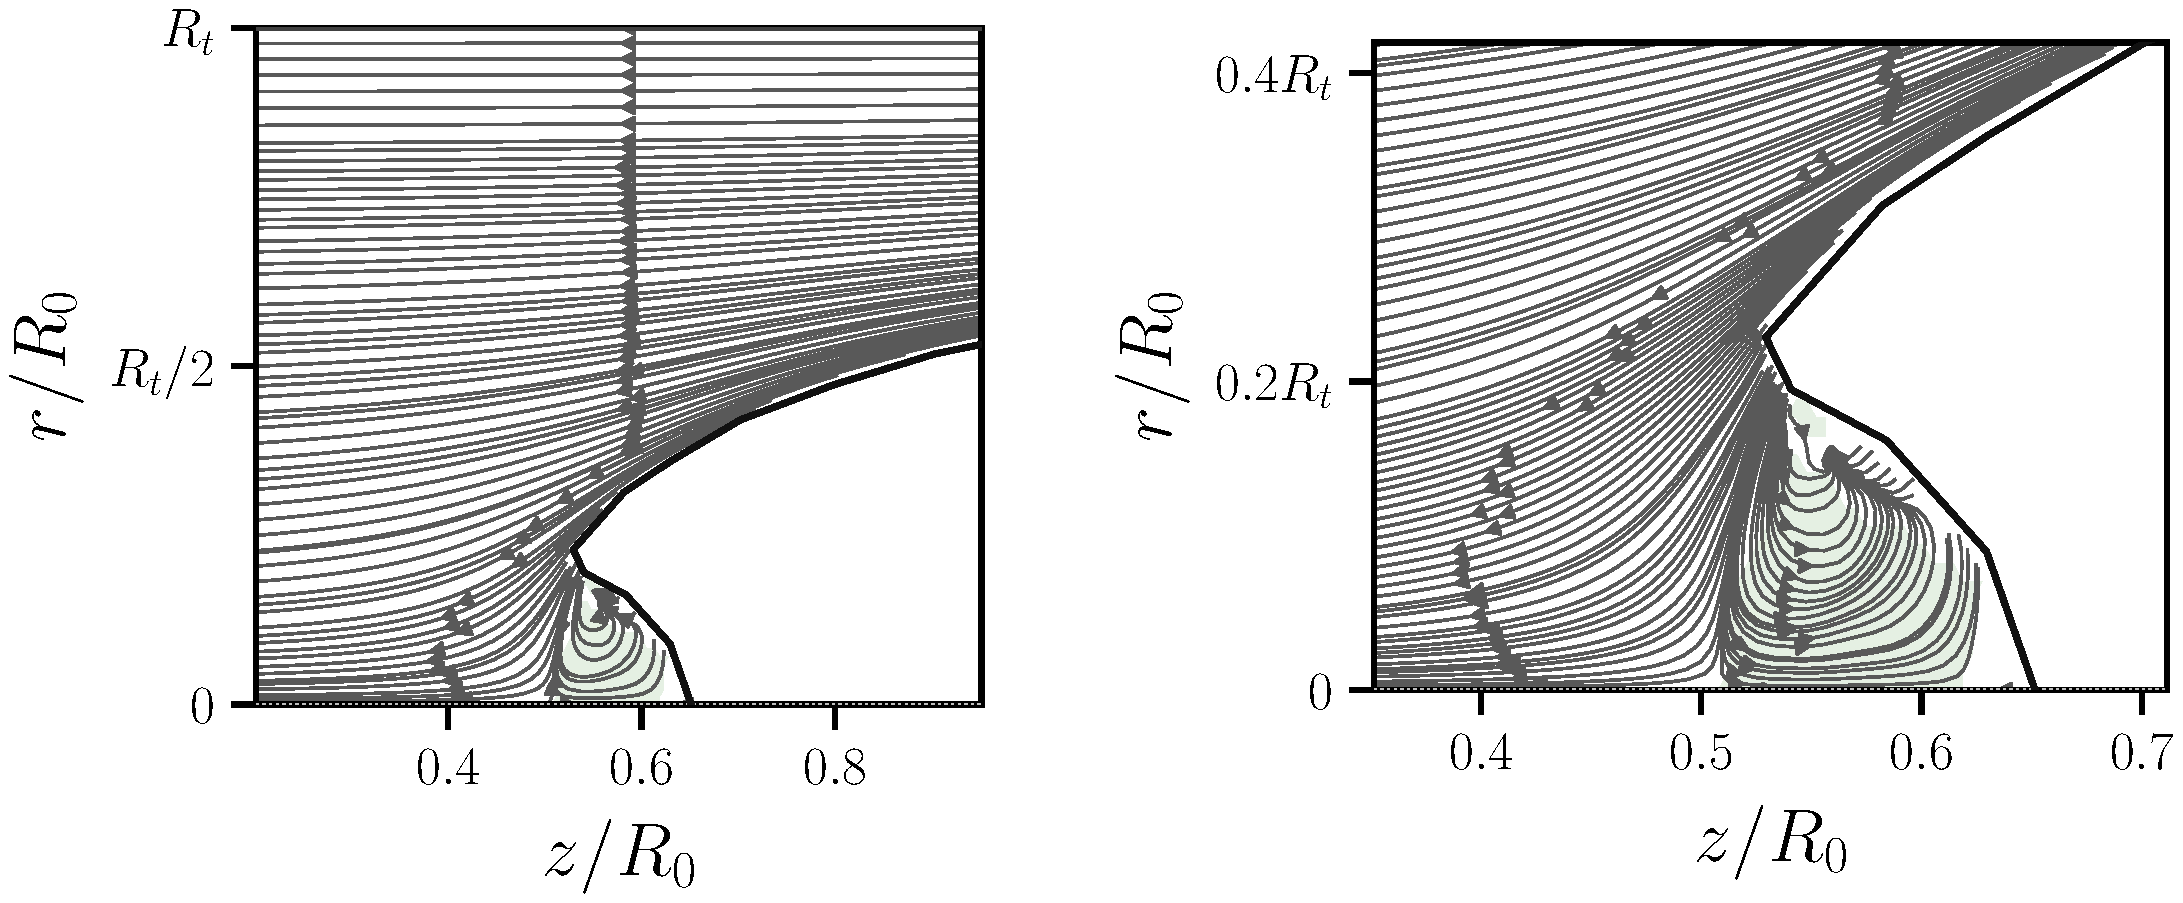
\includegraphics[width=\textwidth]{rear-flow.pdf}
  \caption{Streamlines about the re-entrant rear cap at $Ca_b=9.80$, in the
  frame of the bubble, with the liquid shaded where it moves forward. Left: the
  cap, the deposited film and the wake. Right: the cavity, where the closed
  vortex ring is resolved. The heavy black curve is the interface and the heavy
  line at the top of the left panel is the tube wall, which runs rearward at
  $-U_b$ in this frame. Both panels are one converged solution, the sweep row at
  $Ca_{\mathrm{in}}=4$.}
  \label{fig:rearflow}
\end{figure}

\paragraph{One mechanism was proposed and measured to be wrong.} A natural
explanation is that the film flux, which must be re-injected into the bulk
behind the bubble, converges radially and stagnates on the axis, raising the
pressure there and pushing the interface in. That is testable, because it
predicts the sign of the radial pressure difference. Measuring it requires
care: the axial gradient behind the bubble is about $8Ca_{\mathrm{in}}/R_t^2$
per unit length, of order $67$ at $Ca_b=10$, so sampling the axis and the wall
at stations differing by even $0.02$ manufactures a difference of $1.3$ from
nothing. With the axial trend removed by a local fit in each radial group, and
restricting to stations strictly behind the rearmost point of the interface,
the axis is found to be \emph{below} the near-wall liquid in pressure, by about
$9$ at $0.25R_0$ behind the tip, decaying to $0.2$ by $0.6R_0$ behind. The sign
is opposite to the proposed mechanism, which is therefore rejected. What the
measurement does show is that the tail sits in a strongly non-developed wake:
at $0.5R_0$ behind the tip the annular liquid moves at $-9.1$ in the bubble
frame while the core moves at $-1.7$, relaxing to the fully developed $-1.83$
on the axis within about $0.6R_0$.

A sufficient explanation must also account for the magnitude, and the scaling
gives only a warning rather than an answer. $Ca_b$ compares viscous with
capillary stress on the global scales $U_b$ and $R_t$, so at $Ca_b\simeq10$
there is no reason to expect the deviatoric normal stress on the interface to be
a small correction to the capillary term. That is an expectation about
magnitudes and not a measurement: the local deviatoric stress depends on the
velocity gradient at the interface, which in a cavity where the liquid barely
moves need not follow the global scale at all. Settling the mechanism requires
the full normal-stress balance evaluated along the interface, deviatoric part
included, which this report does not attempt. \citet{balestra2018viscous} had
already established that the viscous normal stresses at the caps cannot be
neglected for $Ca_b>10^{-3}$, so that framing is theirs and not ours; what is
added here is the measurement along the cap rather than at the vertex, an order
of magnitude beyond their range.

A published candidate mechanism exists, and we record it as a candidate rather
than adopt it. \citet{cappello2025superfast} argue that a convergent
stagnation point on the interface corresponds to a locally pushing normal
stress and a divergent one to a locally pulling stress, so the inhomogeneous
normal stress set up by the recirculating flow lowers the curvature near
convergent points; on that reading the rear on-axis stagnation point is the
convergent one, which would be why the rear cap and not the front inverts. It
is consistent with the recirculation we resolve, and we have \emph{not} tested
it: doing so means measuring the stagnation-point structure on the interface
and the normal stress there, which is the same unattempted calculation as
above. The same paper states that rear recirculation in this regime ``appears
as soon as there is an invagination at the back of the bubble'', with the
supporting figure not shown; Figure~\ref{fig:rearflow} is that figure for a
true void at $Ca_b=9.80$.

Two cautions for anyone reading the coincidence of numbers. Bubbles in
viscoelastic liquids develop a rear cusp above a critical capillary number
itself of order one, also at vanishing Reynolds number; that is a constitutive
effect with a negative wake and a hysteretic dependence on bubble volume, and
none of those features is present here. And the regime our high-$Ca_b$ points
occupy, $U_b/\overline U>2$, is the one the recent literature calls
\emph{super-fast}; at $Ca_b=9.80$ the present solution has
$U_b/\overline U=2.45$.

\section{What is established, and what is not}
\label{sec:open}

The following are established by the evidence above. The solver reproduces
Poiseuille flow, the static Laplace pressure, and window and mesh independence
at the stated tolerances. The computed state is an attractor under time
evolution, not merely a fixed point. Its curve does not depend on the route
taken to compute it. In the thin-film limit it recovers Bretherton's film
coefficient to $0.03$--$0.04\%$ and his front-meniscus pressure coefficient to
$0.4\%$, both by extrapolation and neither given to the solver. Over $0.3\le Ca_b\le10$ it
agrees with an independent published axisymmetric computation to about one per
cent, and at three separate capillary numbers to better than $0.2\%$.

The following are not established. The film is validated through $Ca=10$ by
that printed Giavedoni and Saita point. Beyond it the $Ca_b=14.8$ film is an
unvalidated continuation of the same branch: there is no printed table and no
second independent Stokes computation in the bibliography at $Ca_b>10$. The
departure from the Aussillous--Qu\'er\'e fit there is attributed to
extrapolation of the fit, and that attribution is an inference.
The mechanism of the re-entrant rear cap is open, with one candidate measured
and rejected. The difference from the companion volume-of-fluid campaign is
resolved on the present side but its cause is unidentified; of the four
candidates considered, two are eliminated and the remaining two require work on
the companion side. Inertial effects are no longer a single-state caveat: S15
measures $\mathrm{d}H/\mathrm{d}Re$ at $Ca_b=0.068$, $1.06$ and $14.8$, and
the Stokes baseline holds to $0.78\%$ for $Re<1.47$. Continuation in
$Ca_{\mathrm{in}}$ at $La=1$ terminates near $Ca_{\mathrm{in}}=2.91$ both
with automatic remeshing and without it: S17 seeds that row with remesh,
then climbs with remesh suppressed, holds $11104$ degrees of freedom from
$Ca_{\mathrm{in}}=2$ to $2.9$, and dies at the same $Ca_{\mathrm{in}}=2.90851$
as S15. A remesh-off transient seed at $Ca_{\mathrm{in}}=2$ fails before a
state is obtained, so remesh is required to start the row but does not
remove the barrier. The top-of-sweep inertial point is accordingly quoted
at $La=0.1$ rather than $La=1$. S19 fills the named
$(Ca_{\mathrm{in}},La)$ grid. At $Ca_{\mathrm{in}}=0.05$ the $3\times3$ and
$6\times6$ pads agree in $H$ to $7\times10^{-8}$ at $La=0.1$, $1$ and $10$;
$La=10$ there thins the film by $0.253\%$ at $Re=0.679$. At
$Ca_{\mathrm{in}}=0.5$, $La=10$ the film is $5.8\%$ thinner than Stokes
($H=0.295$, $Ca_b=1.006$, $Re=10.1$), so inertia is no longer a perturbation
at that station. The last completed $La=1$ station,
$Ca_{\mathrm{in}}=2.9$, has $H=0.346$ and $Ca_b=6.77$. Allowed failures
remain at $La=10$, $Ca_{\mathrm{in}}=2$ and at the $Ca_{\mathrm{in}}=6$,
$La=0.1$ pad-doubled window. The S15 and S19 rows are not near
the rear-meniscus threshold of \citet{magnini2025stability}: their modified
Weber number is $We_p=We(2-U_b/U_l)^2/2$ with $We=2\rho U_l^2 R_t/\sigma$,
which on the present scales is
$0.7\,La\,Ca_{\mathrm{in}}^2(2-Ca_b/Ca_{\mathrm{in}})^2$. Converted, the three
S15 stations give $We_p=7.2\times10^{-4}$, $2.5\times10^{-3}$ and $0.55$, all
below $We_p^*\approx3.65$ and the last two outside their $Ca_l$ window; the
S19 station at $La=10$, $Ca_{\mathrm{in}}=0.5$ has $We_p=2.5\times10^{-4}$,
so that $5.8\%$ thinning is a Reynolds-number effect, not their rear
threshold. At $Ca_{\mathrm{in}}=2.9$, $La=1$ one has $We_p=0.664$. Our
$We=La\,Ca_b^2$ is a different group; at the top of the sweep it is $21.5$.
Nothing here
addresses drops, for which a true void cannot stand in for the interior phase
and a second meshed phase is required.

\section*{Data}

All campaign quantities plotted or tabulated in this report are supplied as
compact CSV files under \nolinkurl{data/}, and the verification-stage values of
Table~\ref{tab:stages} are read from the stages' JSON receipts under
\nolinkurl{receipts/}. Every figure is regenerated from the CSV files under
\nolinkurl{data/} by the scripts in \nolinkurl{figures/}, without a solver or
a simulation dump. The
digitised points of \citet{giavedoni1997axisymmetric} record the source figure
and the coordinates read; printed values record the page. The companion volume-of-fluid table is reproduced
with that campaign's agreement and carries its own resolution measure and its
outlet-limited flag, both of which are honoured in the figures.

\bibliographystyle{plainnat}
\bibliography{references}

\end{document}
